\documentclass[]{article}
\usepackage[T1]{fontenc}
\usepackage{lmodern}
\usepackage{amssymb,amsmath}
\usepackage{ifxetex,ifluatex}
\usepackage{fixltx2e} % provides \textsubscript
% use upquote if available, for straight quotes in verbatim environments
\IfFileExists{upquote.sty}{\usepackage{upquote}}{}
\ifnum 0\ifxetex 1\fi\ifluatex 1\fi=0 % if pdftex
  \usepackage[utf8]{inputenc}
\else % if luatex or xelatex
  \ifxetex
    \usepackage{mathspec}
    \usepackage{xltxtra,xunicode}
  \else
    \usepackage{fontspec}
  \fi
  \defaultfontfeatures{Mapping=tex-text,Scale=MatchLowercase}
  \newcommand{\euro}{€}
\fi

\usepackage{graphicx}
% use microtype if available
\IfFileExists{microtype.sty}{\usepackage{microtype}}{}
\def\tightlist{}
\ifxetex
  \usepackage[setpagesize=false, % page size defined by xetex
              unicode=false, % unicode breaks when used with xetex
              xetex]{hyperref}
\else
  \usepackage[unicode=true]{hyperref}
\fi
\hypersetup{breaklinks=true,
            bookmarks=true,
            pdfauthor={Arne Beer MN 6489196; Marta Nevermann MN 6419716; Daniel Waller MN 6813853; Julius Hansen MN 6455291},
            pdftitle={Grundlagen der Wissensverarbeitung -- Tutorial 8, Gruppe 4},
            colorlinks=true,
            citecolor=blue,
            urlcolor=blue,
            linkcolor=magenta,
            pdfborder={0 0 0}}
\urlstyle{same}  % don't use monospace font for urls
\setlength{\parindent}{0pt}
\setlength{\parskip}{6pt plus 2pt minus 1pt}
\setlength{\emergencystretch}{3em}  % prevent overfull lines
\setcounter{secnumdepth}{0}

\title{Grundlagen der Wissensverarbeitung -- Tutorial 8, Gruppe 4}
\author{Arne Beer MN 6489196 \and Marta Nevermann MN 6419716 \and Daniel Waller MN 6813853 \and Julius Hansen MN 6455291}
\date{}

\begin{document}
\maketitle


\subsection{Exercise 1.2}\label{exercise-1.2}

\subsection{Exercise 1.3}\label{exercise-1.3}

Die Wahrscheinlichkeit, dass eine einzelne Komponente im Auto kaputt
ist, beträgt 0.1, implizit ergibt sich daraus die unabhängige
Wahrscheinlichkeit von 0.9, dass eine einzelne Komponente funktioniert.
Man kann den Motor in einem Belief-Network darstellen, mit den einzelnen
Komponenten als Knoten.

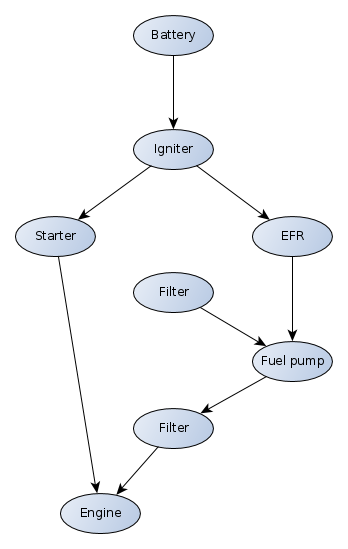
\includegraphics[width=400px]{graph.png}

$
P(\text{Battery})=
\begin{bmatrix}
\textbf{funkt} & \neg\textbf{funkt}\\
0.9 & 0.1
\end{bmatrix}
$

$
P(\text{FT})=
\begin{bmatrix}
\textbf{funkt} & \neg\textbf{funkt}\\
0.9 & 0.1
\end{bmatrix}
$

$
P(\text{Ignition}|\text{Battery})=
\begin{bmatrix}
\textbf{Battery} &\textbf{funkt} & \neg\textbf{funkt}\\
\text{funkt} & 0.81& 0.19\\
\neg\text{funkt}& 0  & 1
\end{bmatrix}
$

$
P(\text{EFR}|\text{Ignition},\text{Battery})=
\begin{bmatrix}
\textbf{Battery} & \textbf{Ignition} &\textbf{funkt} & \neg\textbf{funkt}\\
\text{funkt} & \text{funkt} & 0.729& 0.271\\
\text{funkt} & \neg \text{funkt} & 0 & 1\\
\neg \text{funkt} & \text{funkt} & 0 & 1\\
\neg \text{funkt} & \neg\text{funkt}& 0  & 1
\end{bmatrix}
$

$
P(\text{starter}|\text{Ignition})=
\begin{bmatrix}
\textbf{starter} &\textbf{funkt} & \neg\textbf{funkt}\\
\text{funkt} & 0.729& 0.271\\
\neg\text{funkt}& 0  & 1
\end{bmatrix}
$

$
P(\text{FT}|\text{EFR},\text{FT})=
\begin{bmatrix}
\textbf{EFR} & \textbf{FT} &\textbf{funkt} & \neg\textbf{funkt}\\
\text{funkt} & \text{funkt} & 0.590& 0.409\\
\text{funkt} & \neg \text{funkt} & 0 & 1\\
\neg \text{funkt} & \text{funkt} & 0 & 1\\
\neg \text{funkt} & \neg\text{funkt}& 0  & 1
\end{bmatrix}
$

$
P(\text{Filter}|\text{FP})=
\begin{bmatrix}
\textbf{FP} &\textbf{funkt} & \neg\textbf{funkt}\\
\text{funkt} & 0.531& 0.468\\
\neg \text{funkt} & 0 & 1\\
\end{bmatrix}
$

$
P(\text{eng}|\text{starter},\text{Filter})=
\begin{bmatrix}
\textbf{starter} & \textbf{Filter} &\textbf{funkt} & \neg\textbf{funkt}\\
\text{funkt} & \text{funkt} & 0.348 & 0.651\\
\text{funkt} & \neg \text{funkt} & 0 & 1\\
\neg \text{funkt} & \text{funkt} & 0 & 1\\
\neg \text{funkt} & \neg\text{funkt}& 0  & 1
\end{bmatrix}
$

Die Wahrscheinlichkeit, dass die Batterie voll funktionstüchtig ist, ist: $0.9$.

Die Wahrscheinlichkeit, dass er Anlasser voll funktionstüchtig ist, ist: $0.729$.

Die Wahrscheinlichkeit, dass er Motor voll funktionstüchtig ist, ist: $0.348$.

Die Wahrscheinlichkeit, dass er Motor voll funktionstüchtig ist, ist: $0.656$.

Die Wahrscheinlichkeit, dass der Motor funktioniert, nachdem beobachtet wurde, dass die Pumpe voll funktionstüchtig ist: $0.656$.

\subsection{Exercise 1.4}\label{exercise-1.4}

Gegebene Wahrscheinlichkeiten:

$
P(\text{smuggler})=0.01
$\\
$
P(\text{fever})=0.013
$\\
$
P(\text{dog}|\neg \text{smuggler})=0.05
$\\
$
P(\text{dog}|\text{smuggler})=0.8
$\\
$
P(\text{sweat}|\neg \text{smuggler} \land \neg \text{fever})=0.0
$\\
$
P(\text{sweat}|\neg \text{smuggler} \land \text{fever})=0.6
$\\
$
P(\text{sweat}|\text{smuggler} \land \neg \text{fever})=0.4
$\\
$
P(\text{sweat}|\text{smuggler} \land \text{fever})=0.8
$\\

\includegraphics[width=400px]{exercise1dot4.png}
\\
Folgende Warscheinlichkeiten können berechnet werden:

$
P(\text{sweat})=0.011774
$\\
$
P(\text{dog})=0.0575
$\\

Nach dem Satz von Bayes ergibt sich $P(\text{smuggler}|\text{dog})=P(\text{dog}|\text{smuggler} * P(\text{smuggler}) / P(\text{dog})$,
somit ist $P(\text{smuggler}|{\text{dog})=0.139$.
"Explaining away" ist hier nur auf 'Sweat' anwendbar, ist eine der Bedingungen gegeben, kann die andere ignoriert werden, so ist zum Beispiel bei einem schwitzenden Schmuggler egal ob dieser auch Fieber hat.




\end{document}
